\documentclass[a4paper, oneside]{article}
\usepackage[utf8]{inputenc}
\usepackage[czech]{babel}
\usepackage{amsmath}
\usepackage{amssymb}
\usepackage{amsfonts}
\usepackage{graphicx}
\begin{document}
\author{Bc. František MACH, Ing. Pavel Karban, Ph.D.}
\date{\today}
\title{Agros2D-řešení přestupu tepla ve zdivu}
\maketitle
	Tento seriál navazuje na nedávno publikovanou recenzi Agros2D – aplikace pro řešení fyzikálních polí. V tomto úvodním díle si na příkladu řešení přestupu tepla ve zdivu ilustrativního domu ukážeme základy práce s aplikací.
\tableofcontents
\newpage
\section{Úvod}
	Postup práce v Agros2D lze stejně jako v ostatních programech pro řešení fyzikálních polí rozdělit na preprocessing, processing a postprocessing. V první fázi definování problému (preprocessing) je nutné nejprve vytvořit geometrii (definiční oblast). Agros2D pracuje s třemi elementy, kterými jsou uzel, hrana a značka oblastí. Uzel je základní element, který je nutné využít pro vytvoření hrany (to však neplatí pro práci ve skriptu). V ostatních programech se uzly často nazývají klíčové body (Key Points). Značky oblastí slouží, jak název napovídá, k definování oblasti a platí, že každá uzavřená oblast musí mít právě jednu značku oblasti a to i v případě, že se daná oblast v řešení uvažovat nebude. V další fází je nutné nadefinovat okrajové podmínky a materiály, které se nasledně přiřadí jednotlivým hranám či značkám oblastí.\\
	Řešení problému (processing) zahrnuje diskretizaci (vytvoření výpočetní sítě) a samotné řešení parciálních diferenciálních rovnic, které popisují daný problém. Agros2D k diskretizaci využívá program Triangle \\(http://www.cs.cmu.edu/~quake/triangle.html) založený na Delaunay triangulaci a pro řešení zmíněných rovnic knihovnu Hermes2D \\(http://hpfem.org/hermes2d) využívající adaptivní metodu konečných prvků vyššího řádu přesnosti (hp-FEM). Díky této knihovně získává Agros2D možnost využití automatické hp adaptivity. V dnešním díle se však touto možností výpočtu zabývat nebudeme a vrátíme se k ní v díle příštím.\\
	Řešením daného problému získáme informace o rozložení veličin řešeného pole. Agros2D nabízí samozřejmě také možnost dalšího zpracování výsledků (postprocessing). Je například možné zobrazit různé veličiny příslušného pole pomocí barevných map, vektory těchto veličin, ekvičáry, parametry řešení jako je počáteční a řešená síť nebo řád polynomu v jednotlivých elementech. V praxi je také důležité znát další veličiny, které ze základních veličin řešeného pole vycházejí. Ty je možné v aplikaci vypočítat lokálně nebo integrací přes povrchy a objemy.\\
	Ovládání aplikace nabízí uživatelům více cest jak se dobrat k požadované funkci nebo výsledku a každý uživatel si tak může vybrat svůj způsob ovládání. Lze tedy využívat pouze uživatelského rozhraní (menu, toolbar, kontextové menu pracovní plochy a panelu Problém) a kombinovat tento postup s klávesovými zkratkami (nejčastější se vypisují v panelu Rychlé rady) nebo využít možnosti práce ve skriptu a pomocí příkazů. Práci ve skriptu se však budeme věnovat v dalších dílech seriálu.\\
	Při práci s Agros2D je potřeba se přepínat mezi různými módy (Práce s uzly, Práce s hranami, Práce se značkami oblastí, Postprocessor). Na první pohled se může tento princip zdát nepraktický, ale přináší sebou některé výhody. Můžete například pracovat s více elementy jednoho druhu aniž byste jakkoliv ovlivňovaly elementy jiné. Módy také práci zpřehledňují a usnadňují tak orientaci.\\
	V dnešním díle bude řešen příklad přestupu tepla ve zdivu ilustrativního domu a to s tepelnou izolací i bez ní. Příklad je ilustrativní pouze v jednoduchosti geometrie. Parametry prostředí jsou voleny podle reálných, již provedených, výpočtů. Musím však podotknout, že tato problematika není přímo předmětem našeho zájmu a mohou se vyskytnout určité nepřesnosti. Budeme velmi rádi když nás na ně upozorníte.\\

\begin{figure}[htbp]
\centering
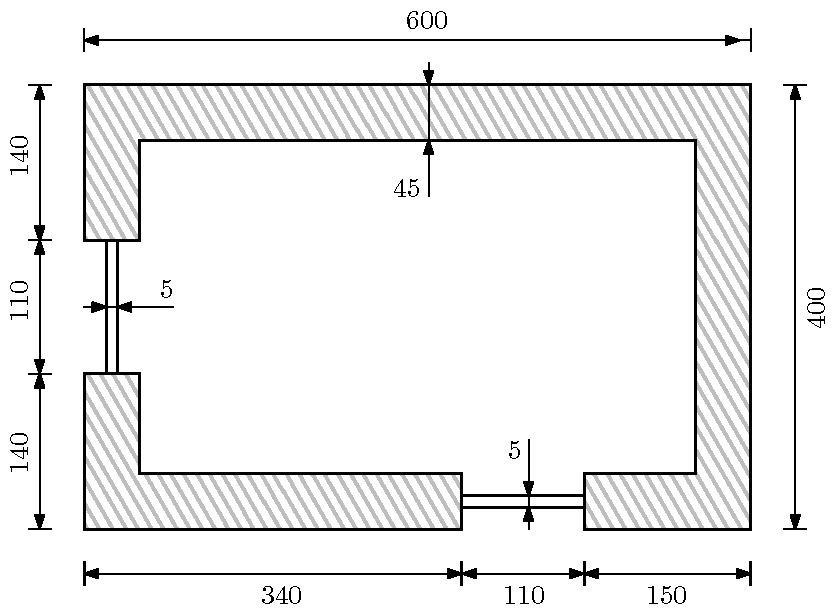
\includegraphics{Nakres.png}\\
\caption{Nákres}
\end{figure}


\begin{figure}[htbp]
\centering
\includegraphics{Matematicky_model.png}\\
\caption{Matematický model}
\end{figure}

\section{Vytvoření nového problému}

	Při spuštění aplikace se vždy vytvoří nový přednastavený problém, který můžete změnit v nastavení aplikace. Před tím, než začnete pracovat je dobré zkontrolovat, zda je právě vytvořený problém nastaven správně a případně jej změnit nebo vytvořit nový. Pomocí příslušné položky v menu Soubor nebo pomocí klávesové zkratky Ctrl+N otevřete dialog nastavení nového problému. Nejdůležitější je nastavení typu řešeného pole, protože po vytvoření problému se již nedá změnit. Pro náš případ zvolíme stacionární teplotní pole a kartézský typ problému. Počet zjemnění ponecháme nastaven na hodnotu 1 a řád polynomu zvyšíme na hodnotu 3. Tyto parametry ovlivňují přesnost řešení, ale podrobné vysvětlení si uvedeme v až příštím díle. Ostatní nastavení problému můžete ponechat ve standardním nastavení.\\
	
\begin{figure}[htbp]
\centering
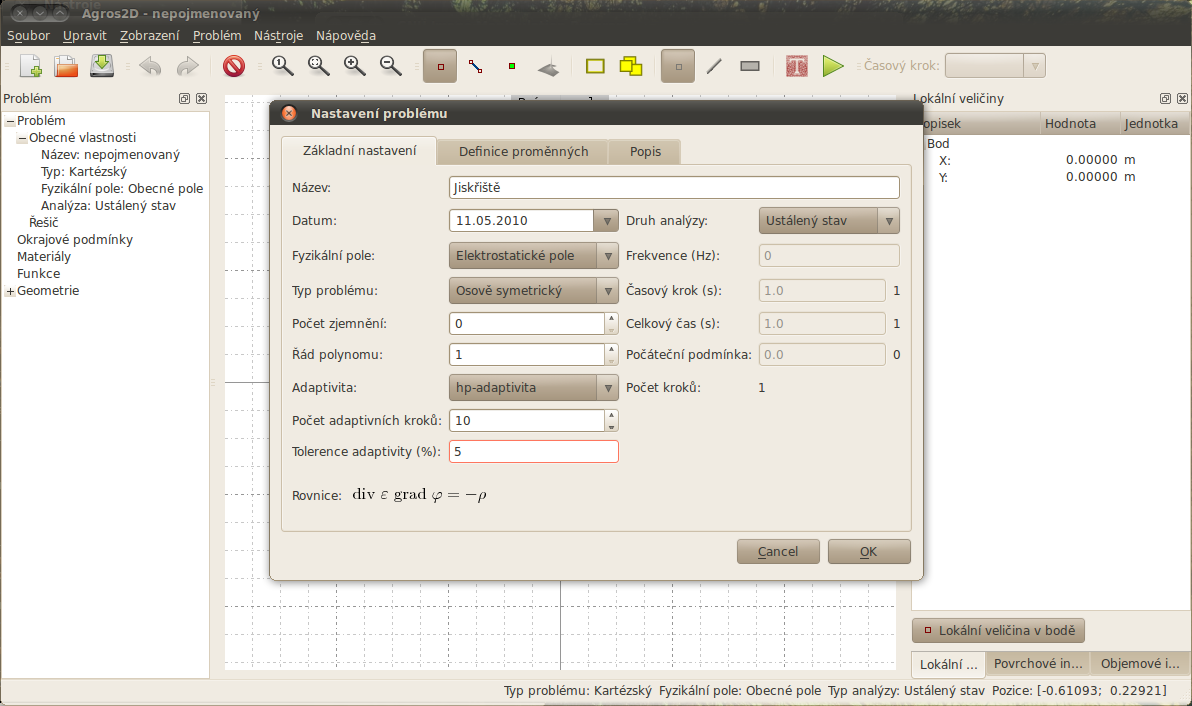
\includegraphics[width=12cm]{Nastaveni_problemu.png}\\
\caption{Nastavení problému}
\end{figure}

\section{Geometrie}
	Jak již bylo řečeno v úvodu, prvním krokem při vytváření geometrie je přidání uzlů. Uzly můžete přidávat hned několika způsoby. Prvním z nich je zádání pomocí přesných souřadnic. Dialogové okno pro jejich zadání můžete vyvolat pomocí klávesové zkratky Alt+N, v kontextového menu pracovní plochy nebo také v panelu Problém. Při zadávání souřadnic můžete využít možnosti vyhodnocování výrazů přímo v textových polích. Tuto možnost můžete využívat v celé aplikaci. Při využívání vyhodnocování výrazů je učelné zapnout v nastavení aplikace na kartě Hlavní zobrazování výsledků textových polí.\\
	Další možností přidání uzlu přímo na pozici kurzoru je pomocí klávesy Ctrl a levého tlačítka myši. U tohoto způsobu můžete s výhodou využít funkce zachytávání do mřížky a také zobrazení pravítka, které si opět můžete zapnout v nastavení aplikace v kartě Zobrazení. Dobrou pomůckou při tvorbě geometrie jsou také transformace, které umožňují posun, rotaci a zvětšení či zmenšení. Pro jejich použití je nutné nejprve vybrat jednotlivé elementy (uzly, hrany nebo značky oblastí) a poté pomocí kontextového menu otevřít dialogové okno umožňující dané funkce využít. Přidáme tedy postupně uzly na následujících souřadnicích.\\

\begin{figure}[htbp]
\centering
	
\begin{tabular}{|c|c|c|c|c|c|c|c|c|c|c|c|c|}
\hline
x(m) & 0 & 6 & 6 & 3.4 & 4.5 & 0 & 0 & 0.45 & 3.4 & 4.5 & 5.55 & 5.55\\
\hline
y(m) & 0 & 0 & 4 & 0 & 0 & 1.4 & 2.6 & 0.45 & 0.45 & 0.45 & 0.45 & 3.55\\
\hline 
\end{tabular} \\
\begin{tabular}{|c|c|c|c|c|c|c|c|c|c|c|}
\hline
 0.45 &0 .45 & 0.45 & 3.4 & 3.4 & 4.5 & 4.5 & 0.2 & 0.25 & 0.2 & 0.25\\
\hline
 3.55 & 1.4 & 2.6 & 0.2 & 0.25 & 0.2 & 0.25 & 2.6 & 2.6 & 1.4 & 1.4\\
\hline 
\end{tabular}
\end{figure}
	Následně musíme uzly propojit pomocí hran. Přepneme se do módu Práce s hranami pomocí klávesové zkratky F6 nebo příslušné položky v menu Problém. Přidání hran můžeme opět provést několika způsoby z nichž nejrychlejší je způsob, kdy pomocí klávesy Ctrl a levého tlačítka myši vyberete vždy dva uzly, které chcete propojit. Další možností je přidání hrany výběrem bodů z nabídky v dialogovém okně, které lze otevřít pomocí klávesové zkratky Alt+E nebo kontextového menu pracovní plochy. Podle obrázku geometrie přidáme všechny hrany. Poslední nutnou fází při vytváření geometrie je vložení značek oblastí. Přepneme se do módu Práce se značkami oblastí pomocí klávesové zkratky F7 nebo příslušného tlačítka v nástrojové liště. Značky oblastí můžeme přidávat stejným způsobem jako uzly - pomocí souřadnic nebo pomocí klávesy Ctrl a myši.\\
	
\begin{figure}[htbp]
\centering
\includegraphics[width=12cm]{Geometrie_bez_izolace.png}\\
\caption{Geometrie bez izolace}
\end{figure}

\section{Okrajové podmínky a materiály}
	
	Agros2D umožňuje definovat proměnné, které lze následně využívat při práci v aplikaci. Toho využijeme a nadefinujeme si parametry okrajových podmínek a materiálů tak, abychom je následně mohli měnit na jediném místě a nemuseli otevírat nastavení každé okrajové podmínky a materiálu zvlášť. Proměnné se definují v okně nastavení problému. Do textového pole na kartě Definice proměnných tedy vložíme následující definice.\\
ALFA\_interier = 4\\
ALFA\_exterier = 25\\
T\_interier = 20\\
T\_exterier = -15\\
LAMBDA\_cihla = 0.6\\
LAMBDA\_sklo = 0.14\\
LAMBDA\_drevo = 0.11\\

	Okrajové podmínky se nastavují pomocí dialogového okna, které lze otevřít pomocí klávesové zkratky Alt+B nebo pomocí kontextového menu pracovní plochy. Každá okrajová podmínka musí mít jednoznačný název.\\
	Přidáme tedy dvě okrajové podmínky, které potřebujeme k popsání námi řešeného problému. První z nich bude Neumannova okrajová podmínka a bude představovat vnitřní okraj zdiva. Nazveme ji například Interiér a přiřadíme jí potřebné parametry jako je koeficientu přestupu tepla (ALFA\_interier) a externí teplotu (T\_interier). Druhá okrajová podmínka je obdobná té první a bude se lišit jen v použitých parametrech (ALFA\_exterier a T\_exterier) a názvu (Exteriér).\\
	
\begin{figure}[htbp]
\centering
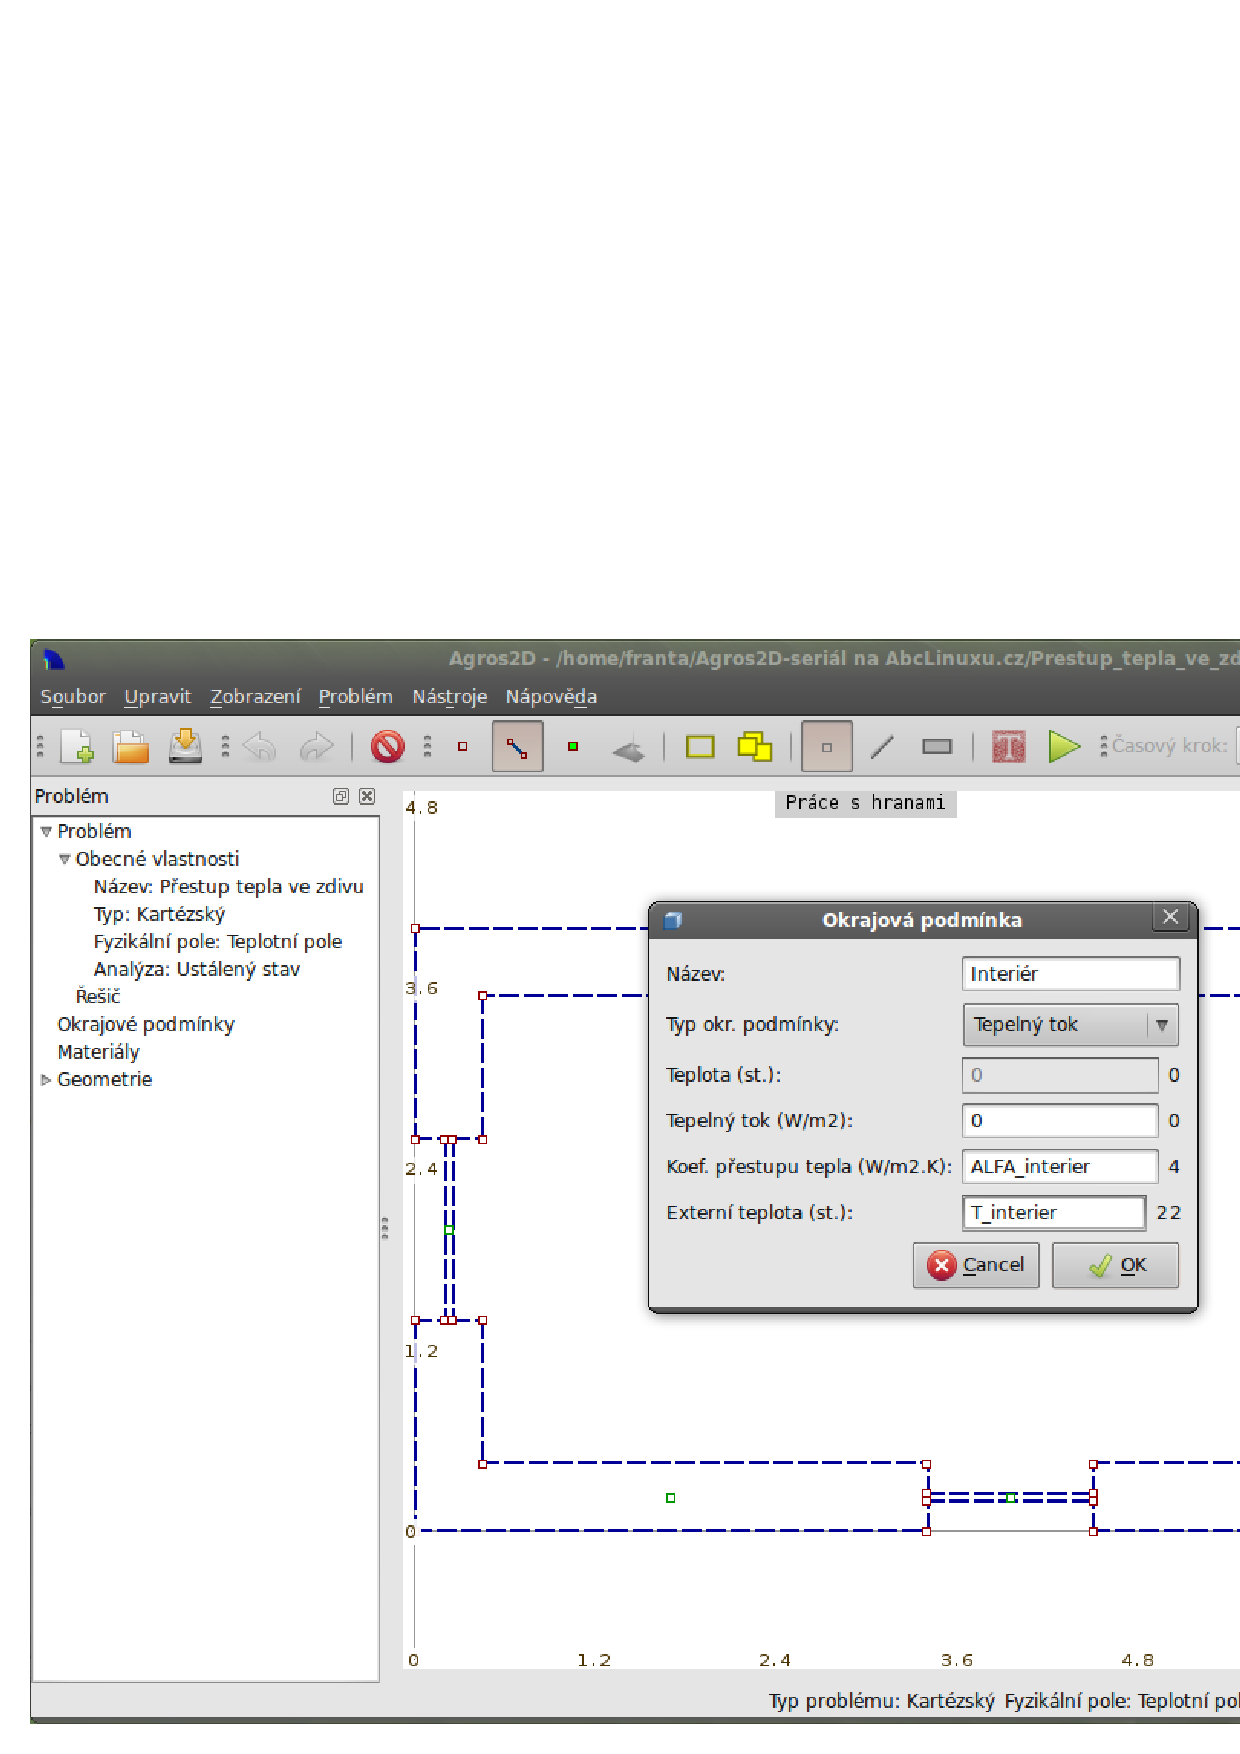
\includegraphics[width=12cm]{Definice_okrajove_podminky.png}\\
\caption{Definice okrajové podmínky}
\end{figure}

	Nadefinované okrajové podmínky je přiřadíme příslušným hranám. Přepneme se do modu Práce s hranami (F6) a vybereme všechny hrany, na kterých platí daná okrajová podmínka a pomocí mezerníku nebo pomocí položky v kontextovém menu vyvoláme dialogové okno a vybereme správnou podmínku. Postupně přiřadíme obě okrajové podmínky na vnitřní (Interiér) i vnější (Exteriér) okraj geometrie. Zda jsou všechny okrajové podmínky přiřazeny správně, si můžete zkontrolovat tak, že danou okrajovou podmínku vybereme ze seznamu v panelu Problém. Po jejím vybrání se označí všechny hrany touto okrajovou podmínku. Rychlou kontrolu také nabízí zobrazení hran, kde plnou čárou se zobrazují hrany s již přiřazenými podmínkami a přerušovanou čárou hrany bez přiřazených podmínek.\\
	
\begin{figure}[htbp]
\centering
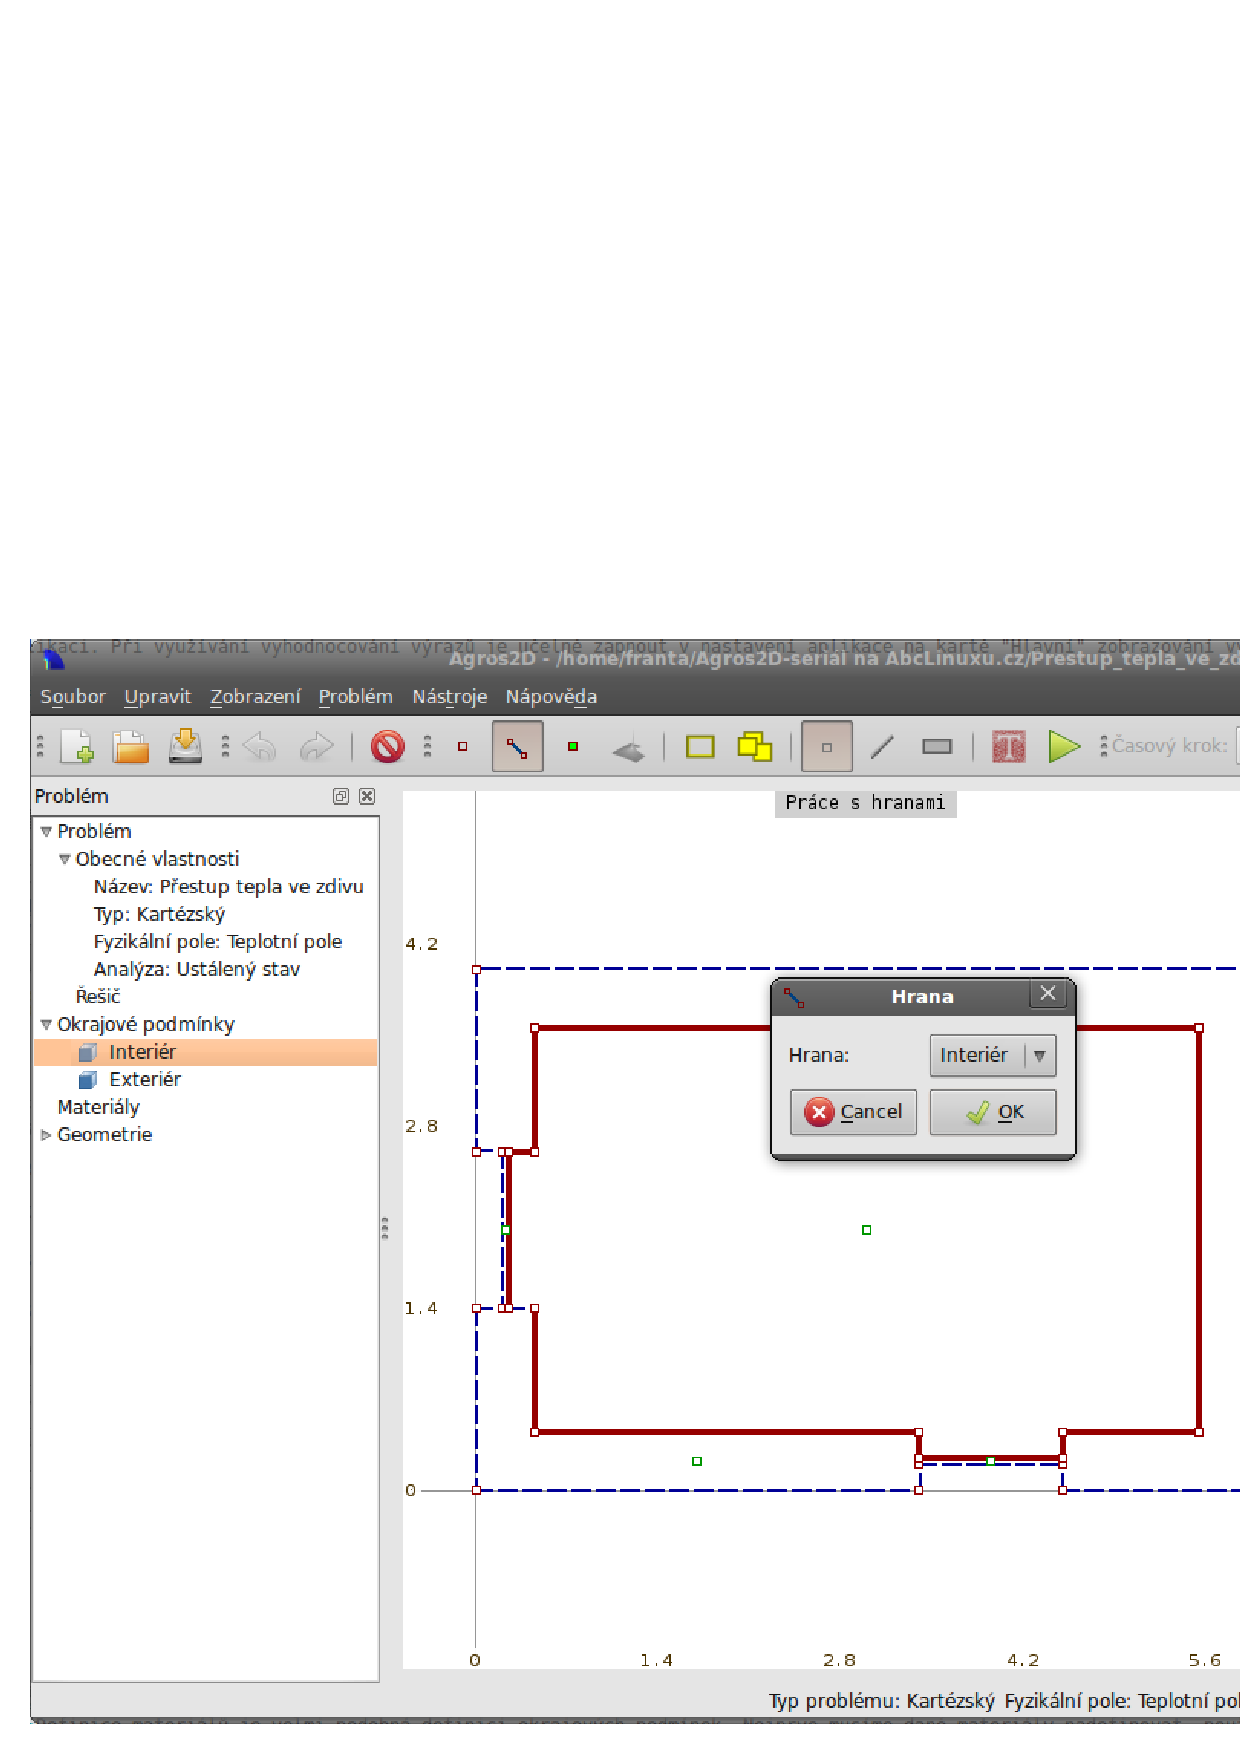
\includegraphics[width=12cm]{Prirazeni_okrajove_podminky.png}\\
\caption{Přiřazení okrajové podmínky}
\end{figure}

	Definice materiálů je velmi podobná definici okrajových podmínek. Nejprve musíme dané materiály nadefinovat. K tomu použijeme klávesovou zkratku Alt+M nebo opět příslušnou položku kontextového menu pracovní plochy a přidáme potřebné materiály (Cihla, Sklo a Dřevo). Těmto materiálům přiřadíme tepelné vodivosti, které jsme si nadefinovali jako proměnné (LAMBDA\_cihla, LAMBDA\_sklo a LAMBDA\_dřevo). Následně definované materiály přiřadíme jednotlivým oblastem. To opět provedeme pomocí mezerníku nebo pomocí položky v kontextovém menu. Vnitřek řešeného domu není součástí problému a rozložení teplotního se zde neřeší. To zařídíme tak, že danou značku oblasti necháme nastavenou na hodnotu none.\\
	
\begin{figure}[htbp]
\centering
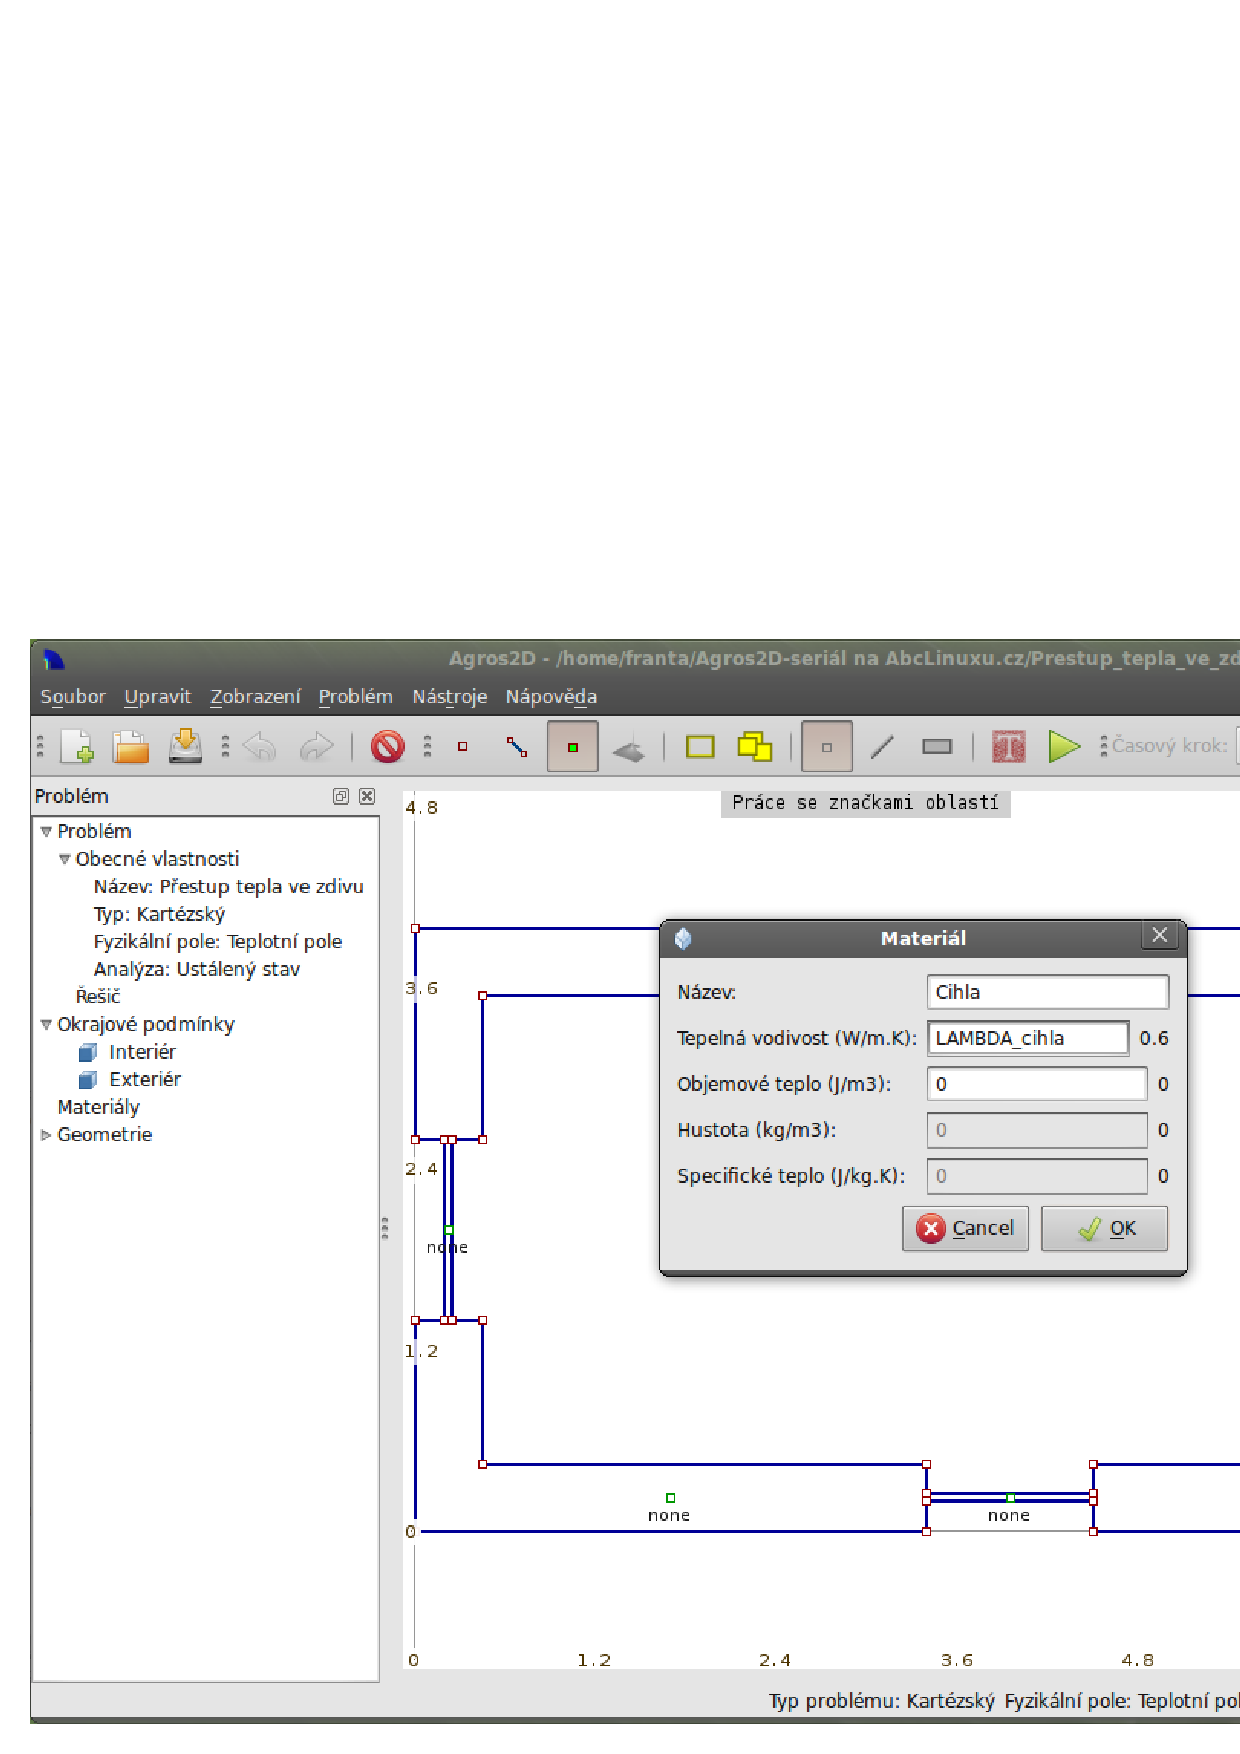
\includegraphics[width=12cm]{Definice_materialu.png}\\
\caption{Definice materialu}
\end{figure}
\newpage
\section{Diskretizace a řešení problému}

	Před samotným výpočtem je vždy dobré nejprve provést diskretizaci, není to ale nutné, protože při spuštění výpočtu se diskretizace provede automaticky. Spustíme tedy diskretizaci pomocí příslušné položky v menu Problém. Pokud diskretizace proběhla v pořádku a zobrazí se síť, tak můžeme přistoupit k samotnému výpočtu. Ten spustíme klávesou Alt+S. Otevře se dialogové okno, kde se vypisují informace o proběhu výpočtu.\\
	
\section{Zpracování výsledků řešení a modifikace problému}
	Po vyřešení problému se aplikace automaticky přepne do režimu Postprocessor a na geometrii se zobrazí barevná mapa průběhu teploty a v pravé části pracovní plochy je zobrazena barevná škála s odpovídajícími hodnotami teploty. Možnosti zobrazení jsou samozřejmě mnohem větší a je možné si je změnit v nastavení scény, které lze otevřít pomocí klávesové zkratky F12, nebo pomocí příslušné nabídky v menu Zobrazení, nebo kontextovém menu pracovní plochy.\\
	Pro náš případ je důležité určit, kolik tepla prochází vnější hranicí zdiva (Exteriér), potřebujeme tedy integrací přes tuto hranici vypočítat celkový tepelný tok. Hrany, po kterých chceme integrovat, můžeme vybrat ručně nebo pomocí funkce výběr podle značky. Obě tyto volby jsou dostupné v menu Problém. Pro náš případ se více hodí automatický výběr. Výsledek výpočtu se zobrazuje v panelu Povrchové integrály. Tepelný tok, který přechází přes hranici oblasti, je 639 W/m.\\
	
\begin{figure}[htbp]
\centering
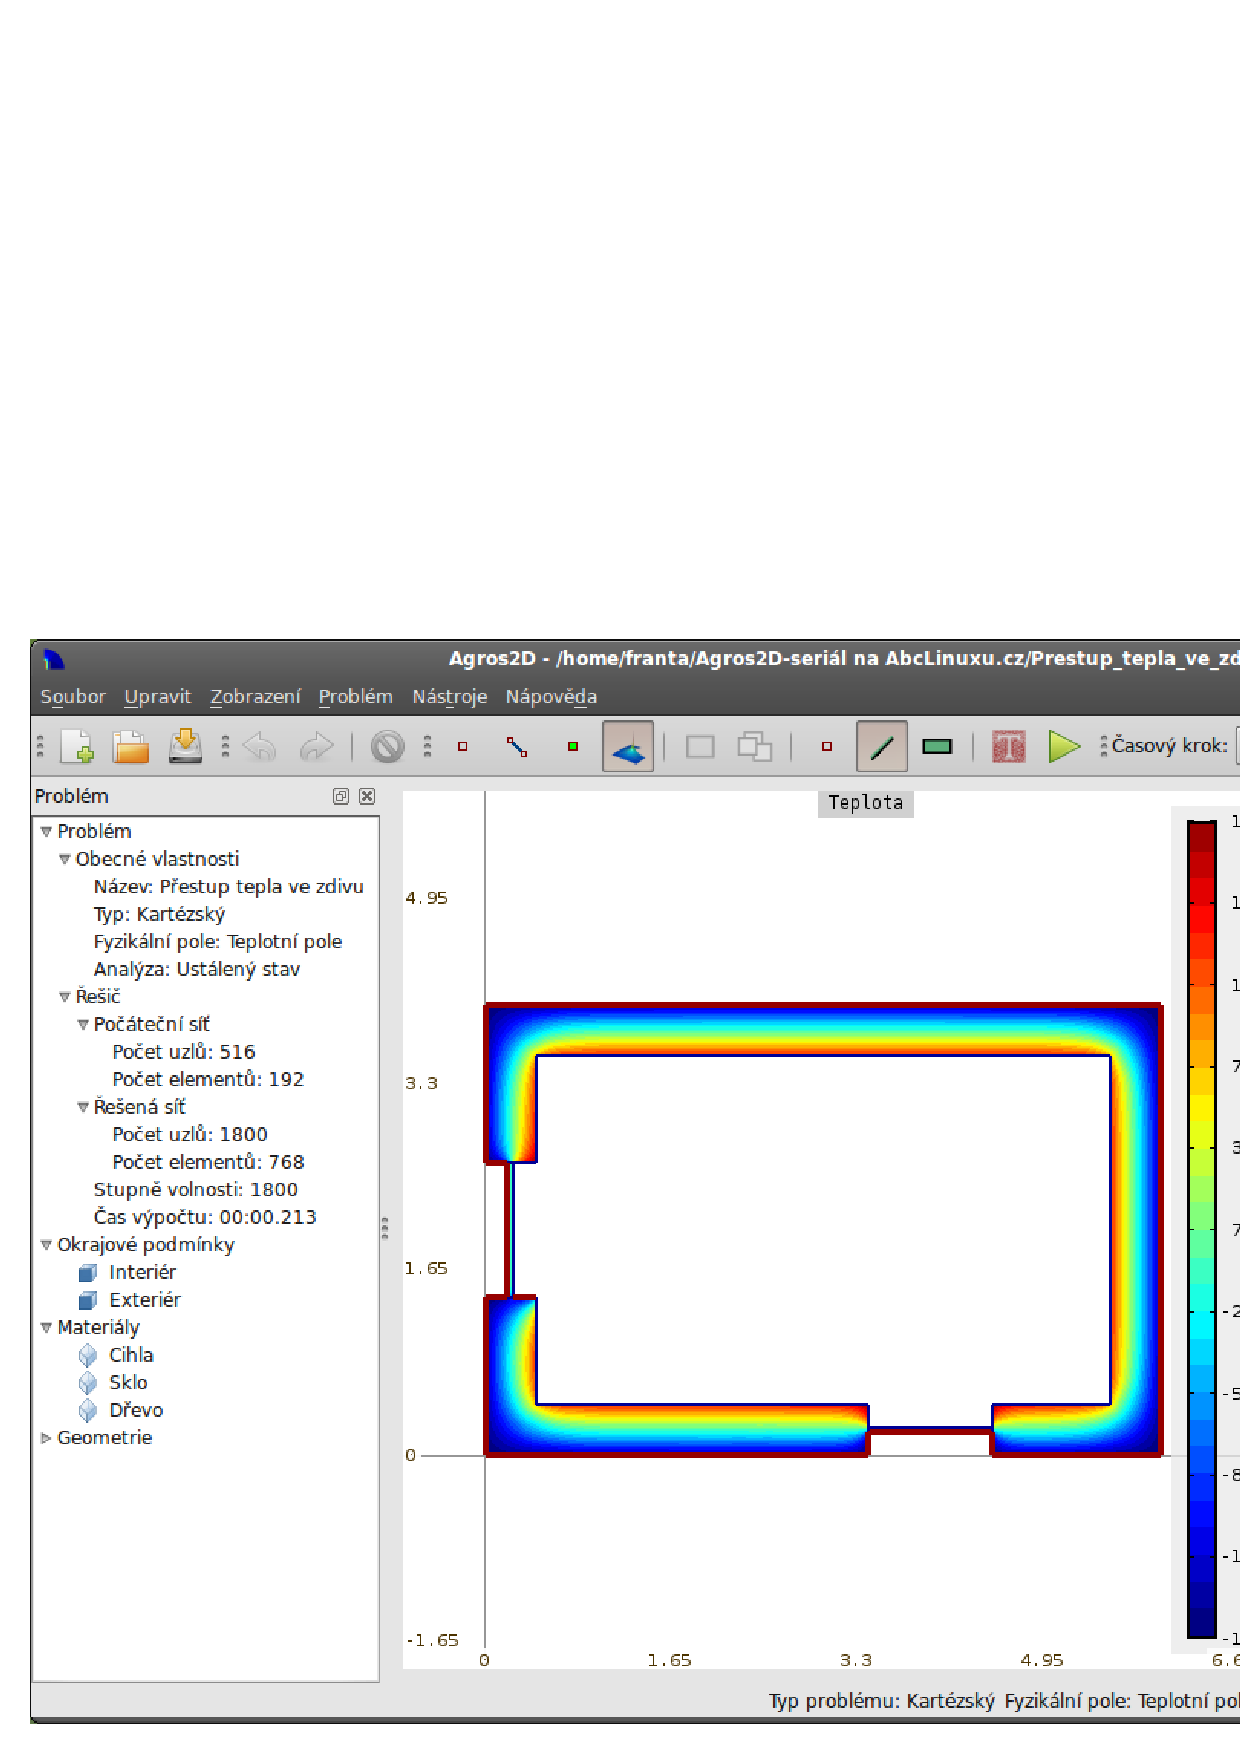
\includegraphics[width=12cm]{Vypocet_tepelneho_toku.png}\\
\caption{Výpočet tepelného toku}
\end{figure}

	Další důležitou věcí, která se při tepelných výpočtech budov sleduje je teplota v průběhu celé stěny a především teplota v rozích místnosti. Podle normy ČSN 73 0540-2 pro vnitřní teplotu $20 ^\circ C$ a venkovní teplotu $-15 ^\circ C$ by tato teplota neměla klesnout pod teplotu $13 ^\circ C$ (zdroj: Katalog tepelných mostů. R. Šubrt, P. Zvánovcová, M. Škopek). Zobrazíme si tedy graf teploty po jedné stěně a zjistíme nejnižší teplotu v celém jejím průběhu. Okno pro kreslení grafu lze otevřít pomocí příslušné položky v menu Nástroje. Nejprve musíme nastavit odkud kam chceme graf vykreslit. Zvolíme například stěnu proti dveřím a zadáme souřadnice počátečního a koncového bodu. Pokud zadáte souřadnice na pracovní ploše hlavního okna se zobrazí úsečka, na které se bude graf kreslit. Můžete si tak lehko zkontrolovat, zda graf zobrazuje to co opravdu chcete. Dalších nastavení si pro tento příklad nemusíme všímnat a můžeme vykreslit průběh teploty.\\
	
\begin{figure}[htbp]
\centering
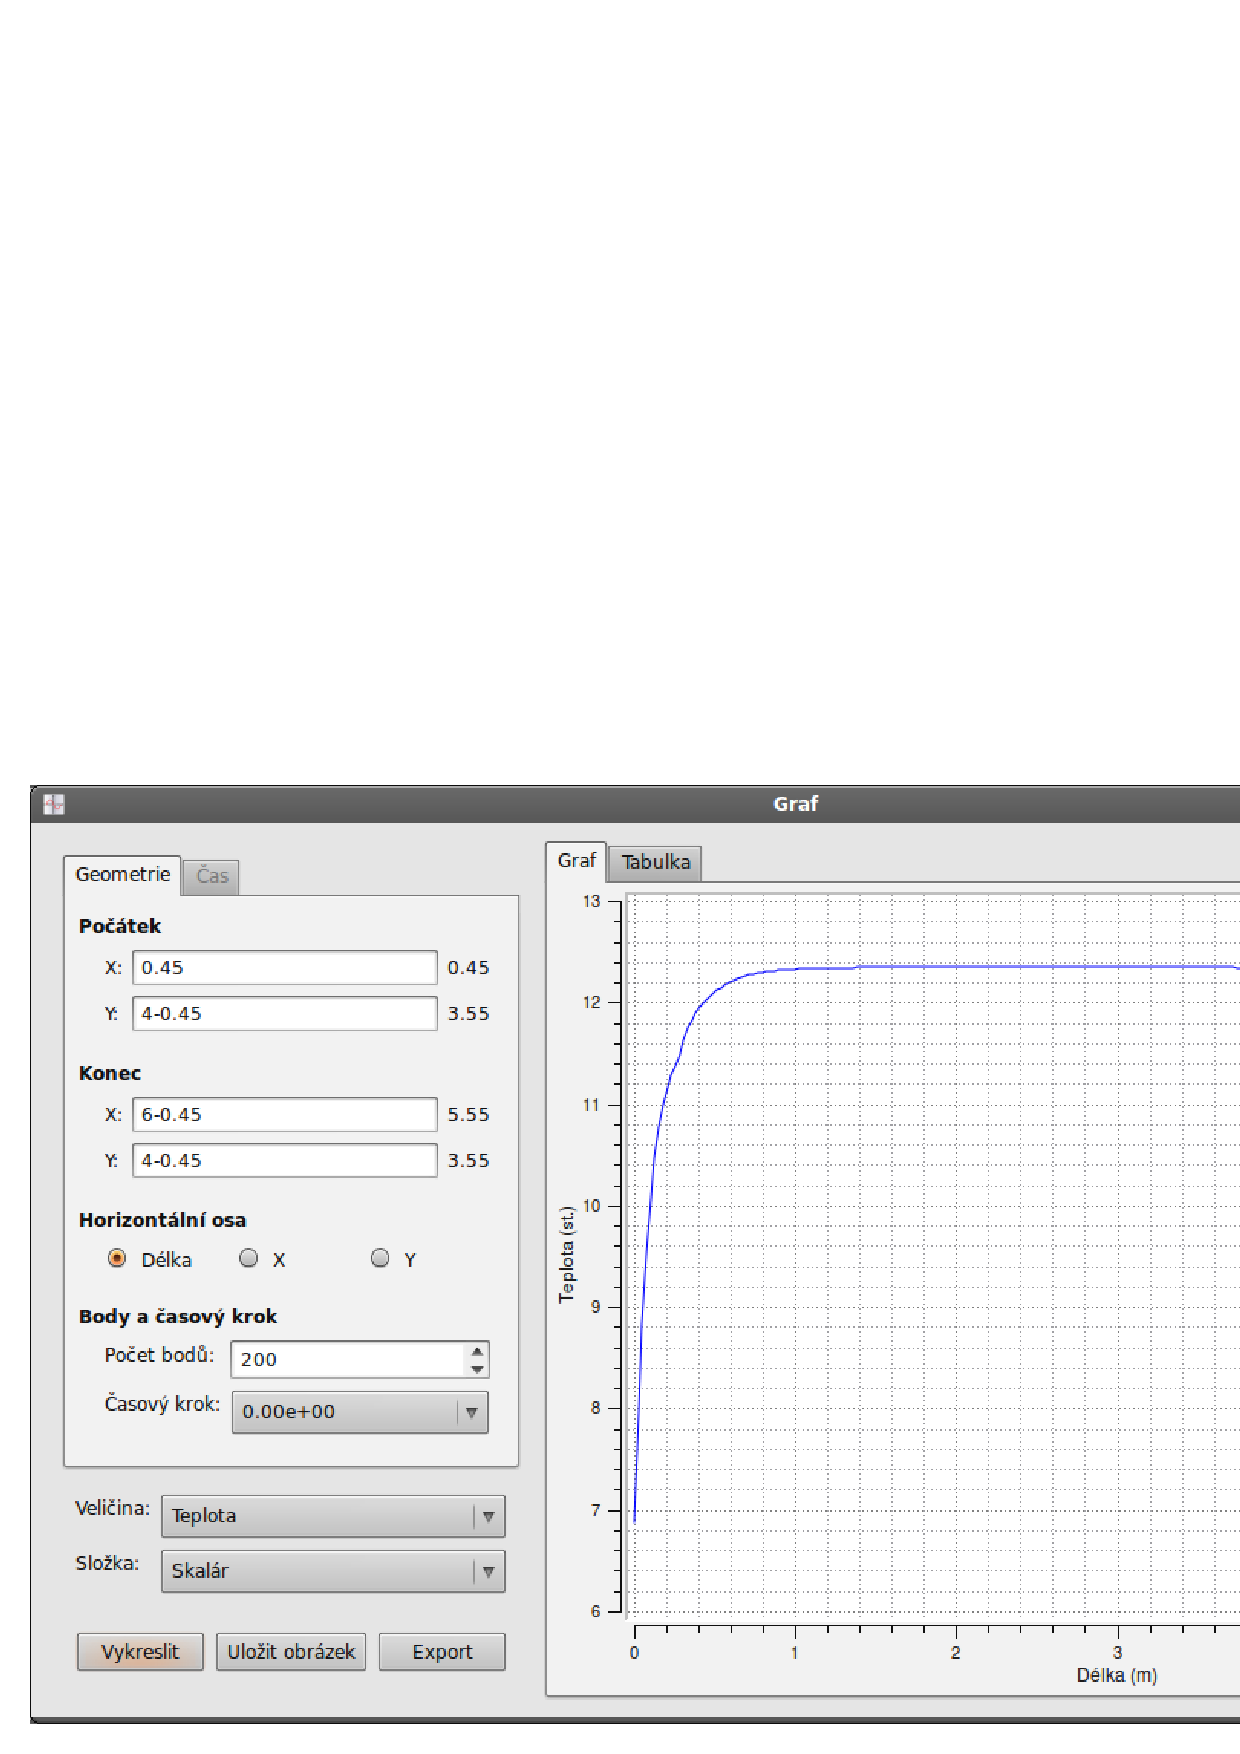
\includegraphics[width=12cm]{Vytvareni_grafu.png}\\
\caption{Vytváření grafu}
\end{figure}

	Z grafu je patrno, že teplota na stěně je mnohem nižší než již uvedené kritérium a to dokonce v celém průběhu. Nyní zkusme spočítat tento příklad s uvažováním izolace o tloušťce 8 cm. Geometrie respektujicí tuto izolaci je již připravená a můžete si ji stáhnout (Prestup\_tepla\_ve\_zdivu\_s\_izolaci.dxf) a naimportovat ze souboru s využitím formátu AutoCAD DXF.\\
	
	Nejprve musíme smazat současnou geometrii. Přepneme se do módu Práce s uzly a vybereme všechny uzly. To můžeme udělat například pomocí klávesové zkratky Ctrl+A nebo v nabídce Problém. Po vybrání uzlů sítě můžeme je smazat pomocí klávesy Del nebo pomocí příslušné položky v nabídce Upravit. Dojde ke smazání uzlů a hran, ale značky oblastí zůstanou. Toho využijeme, abychom nemuseli tyto značky přidávat znovu.\\
	
\begin{figure}[htbp]
\centering
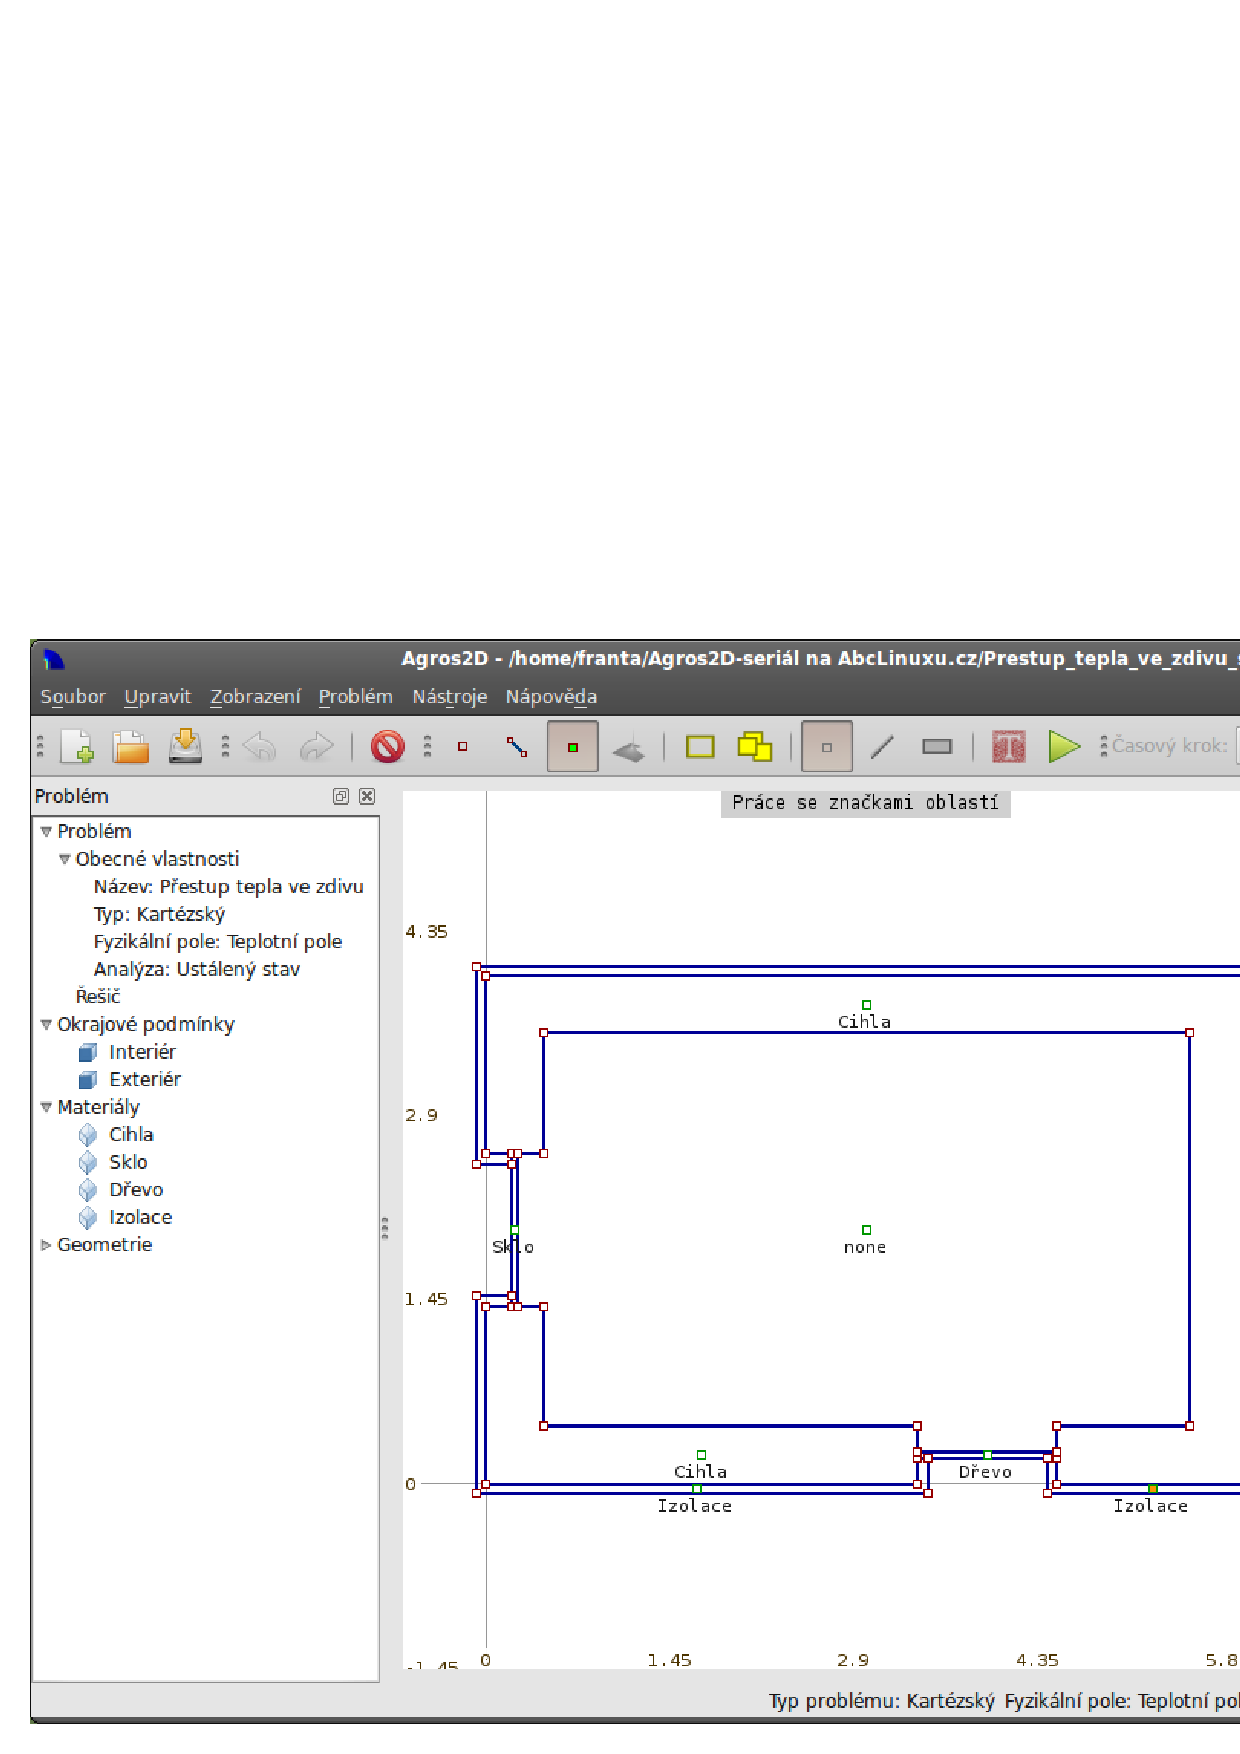
\includegraphics[width=12cm]{Geometrie_izolace.png}\\
\caption{Geometrie s izolací}
\end{figure}

	Nyní naimportujeme novou geometrii úlohy ze staženého souboru pomocí příslušné položky v menu Soubor. Nově vzniklým oblastem musíme přiřadit značky oblastí a materiály. Přidáme si tedy novou proměnnou v nastavení problému, která bude respektovat teplotní vodivost izolace a nadefinujeme a přiřadíme nový materiál (Izolace).\\
	
LAMBDA\_izolace = 0.04\\
	
	Příklad vyřešíme a znovu provedeme výpočet tepelného toku přes vnější hranici geometrie a vykreslení grafu teploty na již dříve vyšetřované stěně. Tepelný tok je pro tento případ roven 302 W/m a je tedy zhruba poloviční oproti případu bez izolace (639 W/m). Z grafu je patrné, že teplota v celém průběhu ani v kritických rozích neklesá pod $13^\circ C$. Zvolená izolace tak výrazně zlepšila zateplení budovy.\\
	
\begin{figure}[htbp]
\centering
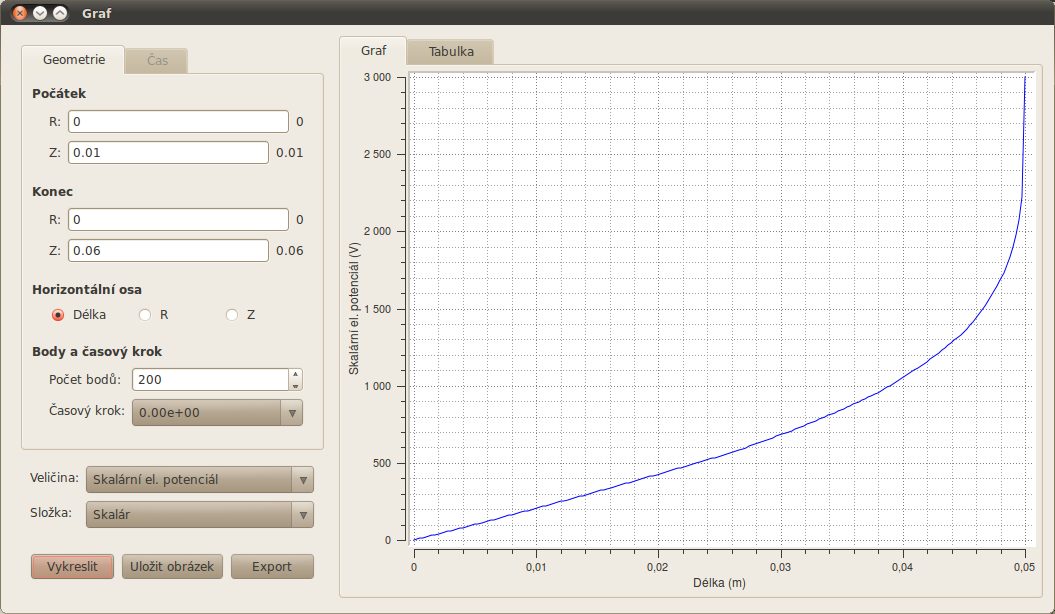
\includegraphics[width=12cm]{Graf.png}\\
\caption{Graf}
\end{figure}

	Oba dnes řešené příklady si můžete stáhnout (Prestup\_tepla\_ve\_zdivu.a2d,\\ Prestup\_tepla\_ve\_zdivu\_s\_izolaci.a2d). V příštím dílu seriálu se budeme zabývat příkladem z oblasti elektřiny a magnetismu. Díl bude zaměřen především na samotné řešení problémů a budeme se také zabývat objasněním využitých výpočetních metod (hp-FEM) a možnostmi automatické hp adaptivity.
\end{document}